\section{Задание №4}

\begin{enumerate}
        \item Построить датчик распределения Коши.
        \item На основе датчика распределения Коши с помощью метода фон Неймана построить датчик стандартного нормального распределения. При помощи функции \texttt{normal probability plot} убедиться в корректности работы построенного датчика и обосновать наблюдаемую линейную зависимость.
        \item Сравнить скорость моделирования стандартного нормального распределения в заданиях 3 и 4.
\end{enumerate}


\subsection{Построение датчика распределения Коши}

\begin{definition}
        Будем говорить, что случайная величина $X$ \textit{имеет распределение Коши с параметрами $a$ и $b$}, если ее функция распределения имеет вид:
$$
        F_X(x) = \frac{1}{\pi}\arctg\left(\frac{x-a}{b}\right) + \frac{1}{2}.
$$ 
        Будем обозначать такие случайные величины
$$
        X \sim \mbox{C}(a,\,b).
$$
\end{definition}

Функция распределения Коши имеет обратную, поэтому воспользовавшись методом обратной функции распределения (смотри теорему \ref{th:inv-method}), получим
$$
        X = F_X^{-1}(\xi) = a + b \tg\left[\pi(\xi - \nicefrac{1}{2})\right],
        \quad
        \mbox{где } \xi \sim \mbox{U}[0,\,1].
$$


\subsection{Построение датчика стандартного нормального распределения методом фон Неймана}

Метод фон Неймана заключается в моделировании нормального распределения путем мажорирования плотностью распределения Коши с параметрами $a$ и $b$. Для достижения наилучшей оценки, будем подбирать значения параметров $a$ и $b$. Выпишем плотности стандартного нормального распределения и распределения Коши:
$$
        \rho_N(x) = \frac{1}{\sqrt{2\pi}} e^{-\frac{x^2}{2}},
$$
$$
        \rho_C(x) = \frac{1}{\pi}\cdot\frac{b}{(x-a)^2+b^2}.
$$
При моделировании будем использовать следующий алгоритм:
\begin{enumerate}
        \item возьмем некоторое число $k > 0$ такое, что $\rho_N(x) \leqslant k \rho_C(x)$ $\forall x \in \R$;
        \item рассмотрим значение случайной величины $\hat\xi = \xi$, где $\xi \sim \mbox{C}(a,\,b)$;
        \item сгенерируем случайную величину $\hat\eta = \eta$, где $\eta \sim \mbox{Bern}\left(\frac{\rho_N(\hat\xi)}{k\rho_C(\hat\xi)}\right)$;
        \item если $\hat\eta = 1$, то $\hat\xi$ является значением случайной величины из распределения с плотностью $\rho_N(x)$, иначе, продолжаем моделирование, начиная с пункта 2.
\end{enumerate}

Данный алгоритм работает тем быстрее, чем ближе отношение $\frac{\rho_N(x)}{k\rho_C(x)}$ к единице, поэтому в качестве $k$ возьмем $k^* = \min\limits_{a,\,b}\max\limits_{x}\frac{\rho_N(x)}{\rho_C(x)}$. Рассмотрим это отношение:
$$
        \frac{\rho_N(x)}{\rho_C(x)}
        =
        \frac{\sqrt{\pi}}{b\sqrt{2}}
        \cdot
        e^{-\frac{x^2}{2}}
        \cdot
        [(x - a)^2 + b^2].
$$
Допустим, что оптимальное значение параметра $a = 0$. Рассмотрим вспомогательную функцию
$$
        g(x) = e^{-\frac{x^2}{2}}(x^2 + b^2)
$$
и найдем ее точки максимума:
$$
        g'(x) = xe^{-\frac{x^2}{2}}(2 - b^2 - x^2)
        \Longrightarrow
        \left[\begin{aligned}
                x = 0, \quad |b| > \sqrt {2}, \\
                x = \pm \sqrt{2 - b^2}, \quad 0 < |b| \leqslant \sqrt{2},
        \end{aligned}\right.
$$
Следовательно,
$$
        k^* = \min\left\{
        \min\limits_{|b| > \sqrt{2}} \sqrt{\frac{\pi}{2}}b,\, \min\limits_{0 < |b| \leqslant \sqrt{2}} \frac{\sqrt{2\pi}}{b} e^{\frac{b^2}{2} - 1}
        \right\}.
$$
Поскольку $k> 0$ и $b > 0$, то найдем минимум еще одной вспомогательной функции:
$$
        h(b) = \frac{e^{\frac{b^2}{2}-1}}{b},\quad h'(b) = \frac{1-b^2}{b^2} e^{\frac{b^2}{2}-1}
        \Longrightarrow b = 1.
$$
Таким образом, при $a^* = 0$, $b^* = 1$:
$$
        k^* = \min\left\{
        \sqrt{\pi},\,
        \sqrt{\frac{2\pi}{e}}
        \right\}
        =
        \sqrt{\frac{2\pi}{e}}.
$$
Напоследок покажем, что $a^* = 0$ действительно является оптимальным значением параметра:
\begin{multline*}
        k^*
        =
        \min\limits_{a,\,b}\max\limits_{x}\frac{\rho_N(x)}{\rho_C(x)}
        =
        \min\limits_{a,\,b}\max\limits_{x} \frac{\sqrt{\pi}}{b\sqrt{2}}
        \cdot
        e^{-\frac{x^2}{2}}
        \cdot
        [(x - a)^2 + b^2]
        = \\ =
        \min\limits_a \left\{
                \min\limits_{b > \sqrt{2}} \left.
                \frac{\rho_N(x)}{\rho_C(x)}
                \right|_{x = 0},\,
        \min\limits_{0 < b \leqslant \sqrt{2}} \left.
                \frac{\rho_N(x)}{\rho_C(x)}
                \right|_{x = \pm \sqrt{2 - b^2}}
        \right\}
        >\\>
        \min\limits_a \left\{
                \min\limits_{b > \sqrt{2}}
                \frac{\sqrt{\pi}}{b\sqrt{2}}(a^2 + b^2),\,
        \min\limits_{0 < b \leqslant \sqrt{2}} 
                (\sqrt{2 - b^2} + |a|)
        \right\}.
\end{multline*}
Минимум же последнего выражения достигается при $a = 0$.


\subsection{Дополнительно о методе фон Неймана}

Проиллюстрируем результат работы датчика при помощи функции \texttt{normal probability plot}. Данная функция строит график распределения в следующих осях: на оси абсцисс откладываются точки выборки, а на оси ординат --- квантили стандартного нормального распределения.

Рассмотрим случайную величину $X \sim \mbox{N}(\mu,\,\sigma^2)$. Тогда ее функция распределения
$$
        F_X(x) = \frac{1}{\sqrt{2\pi\sigma^2}}\int\limits_{-\infty}^{x} e^{-\frac{(t - \mu)^2}{2\sigma^2}}\,dt.
$$
Произведем замену переменной $s = \frac{t - \mu}{\sigma}$, тогда
$$
        F_X(x) = \frac{1}{\sqrt{2\pi}} \int\limits_{-\infty}^{\frac{x - \mu}{\sigma}} e^{-\frac{s^2}{2}}\,ds
        =
        F_N\left(\frac{x - \mu}{\sigma}\right),
$$
где $F_N(x)$ --- функция стандартного нормального распределения.

Получается, что квантили различных нормальных распределений связаны между собой линейно. То есть любая случайная величина $X \sim \mbox{N}(\mu,\,\sigma^2)$ представима в виде $X = \sigma Y + \mu$, где $Y \sim \mbox{N}(0,\,1)$.

Функция \texttt{normal probability plot} для каждой нормально распределенной выборки должна показать прямую со сдвигом $\mu$ и угловым коэффициентом $\sigma$.

В конце хотелось бы сравнить скорости работы моделирования стандартной нормальной случайной велиины при методах моделирования парами (смотри предыдущее задание) и фон Неймана. Для этого мы приведем график скорости работы каждого метода в зависимости от объема генерируемой выборки. Стоит отметить, что программное решение задачи написано в системе \texttt{Matlab}, где на системном уровне реализованы матричные вычисления, которые работают  гораздо быстрее циклов. Метод моделирования парами работает использует только матричные операции, в то время как в методе фон Неймана используется цикл. К тому же матричных операций в методе фон Неймана также используется больше.

\clearpage
\begin{figure}[t]
        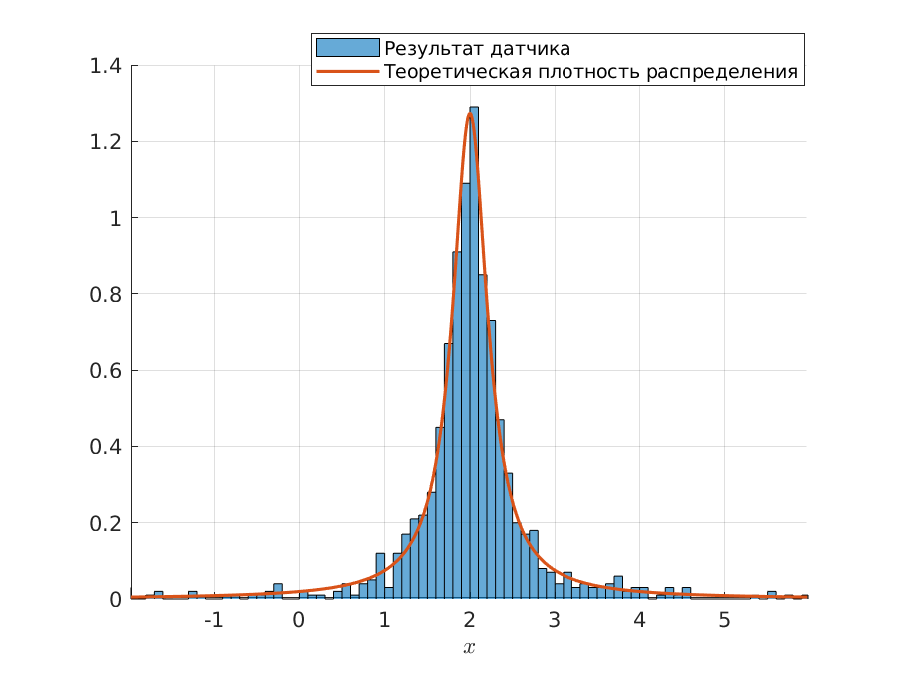
\includegraphics[width=0.5\linewidth]{task_04/c2-025-1000.eps}
        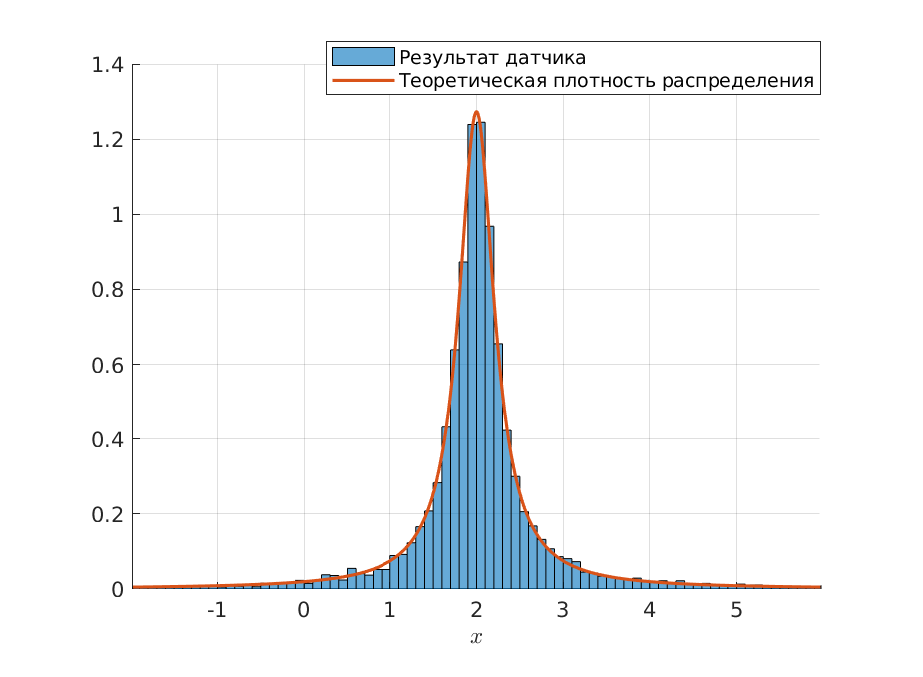
\includegraphics[width=0.5\linewidth]{task_04/c2-025-10000.eps}
        \caption{Гистограмма распределения Коши случайной величины с параметрами $a = 2$ и $b = \nicefrac{1}{4}$ при $10^3$~(слева) и $10^4$~(справа) испытаний.}
\end{figure}
\begin{figure}[b]
        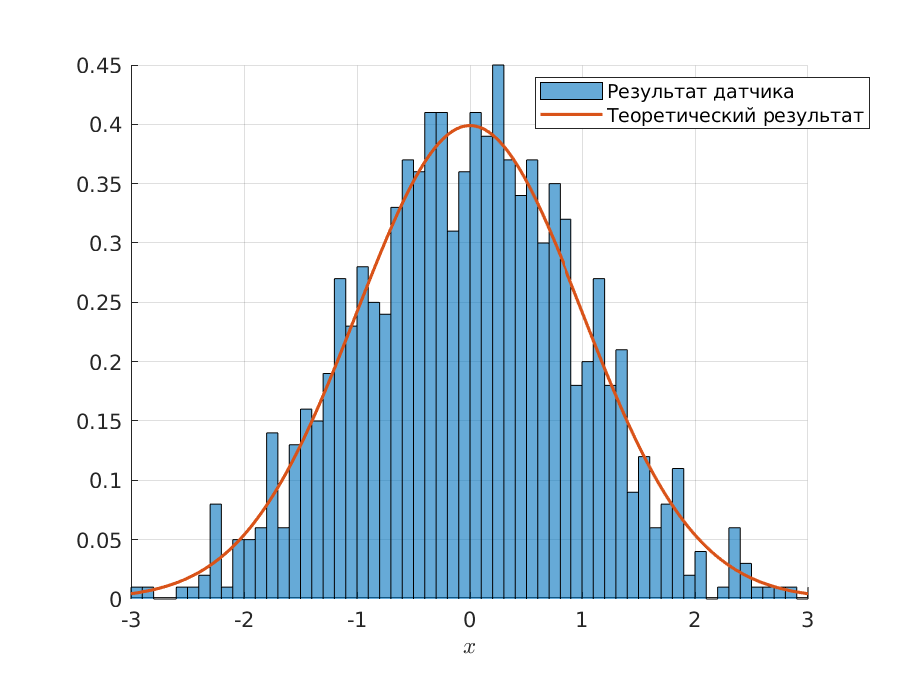
\includegraphics[width=0.5\linewidth]{task_04/von1000.eps}
        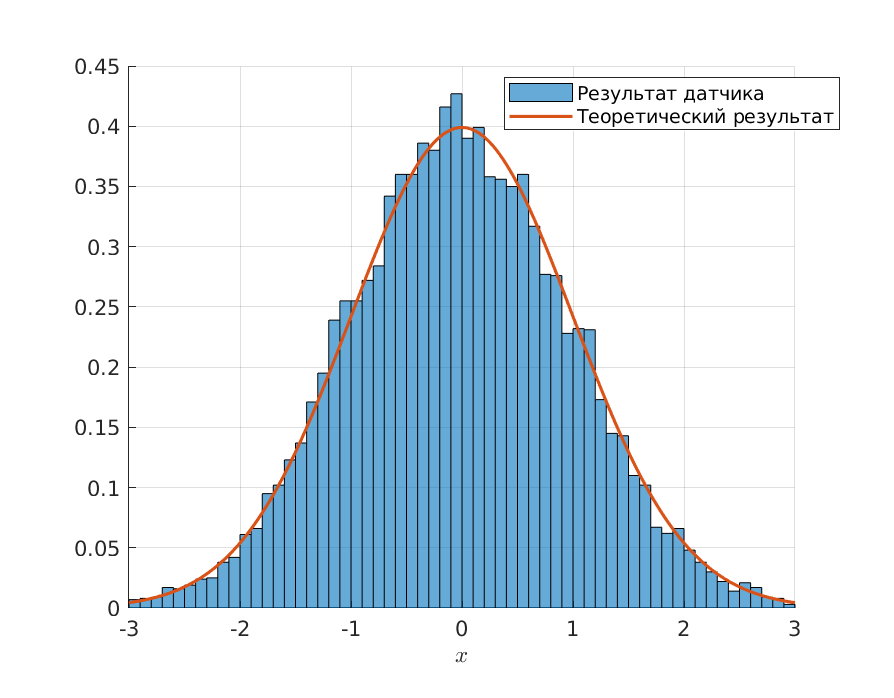
\includegraphics[width=0.5\linewidth]{task_04/von10000.eps}
        \caption{Гистограмма стандартного нормального распределения случайной величины, смоделированной методом фон Неймана при $10^3$~(слева) и $10^4$~(справа) испытаний.}
\end{figure}
\begin{figure}[t]
        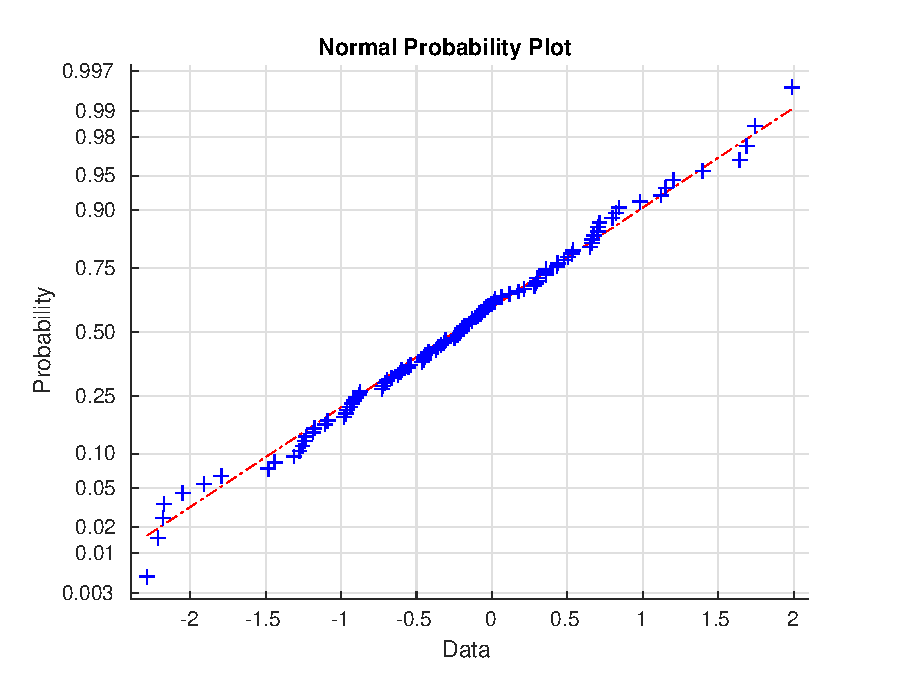
\includegraphics[width=0.5\linewidth]{task_04/norm100.eps}
        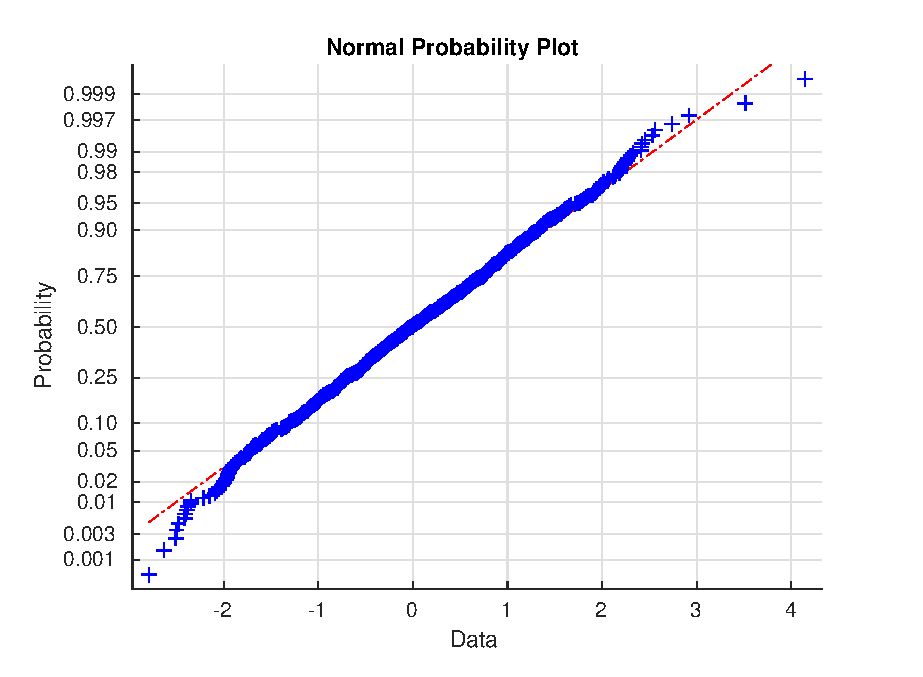
\includegraphics[width=0.5\linewidth]{task_04/norm1000.eps}
        \caption{Результат работы функции \texttt{nornal probability plot} для датчика стандартного нормального распределения методом фон Неймана при $10^2$~(слева) и $10^3$~(справа) испытаний.}
\end{figure}
\begin{figure}[b]
        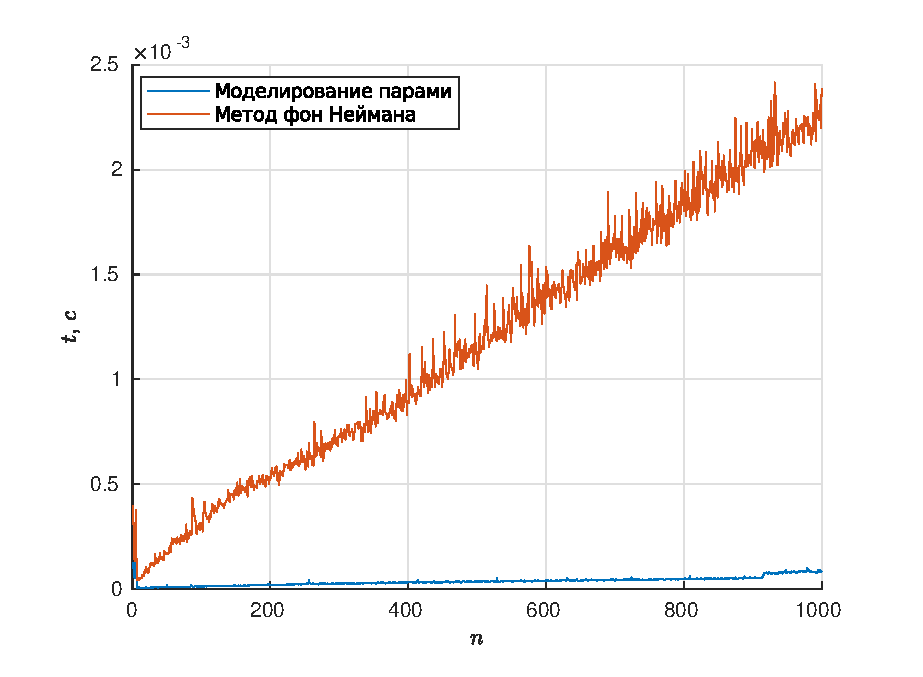
\includegraphics[width=\linewidth]{task_04/speed.eps}
        \caption{Сравнение времени работы методов моделирования стандартного нормального распределения в зависимости от объема выборки.}
\end{figure}